\section{Introduction}
\label{sec:introduction}

\paragraph{} The objective of this laboratory assignment is to design an Audio Amplifier, this is a device that can increase the power of a 
signal so it can be transmited (in our case a voltage that varies with time).

\paragraph{} The architecture chosen for the lab is the one detailed bellow.

\begin{figure}[h]
	\centering
	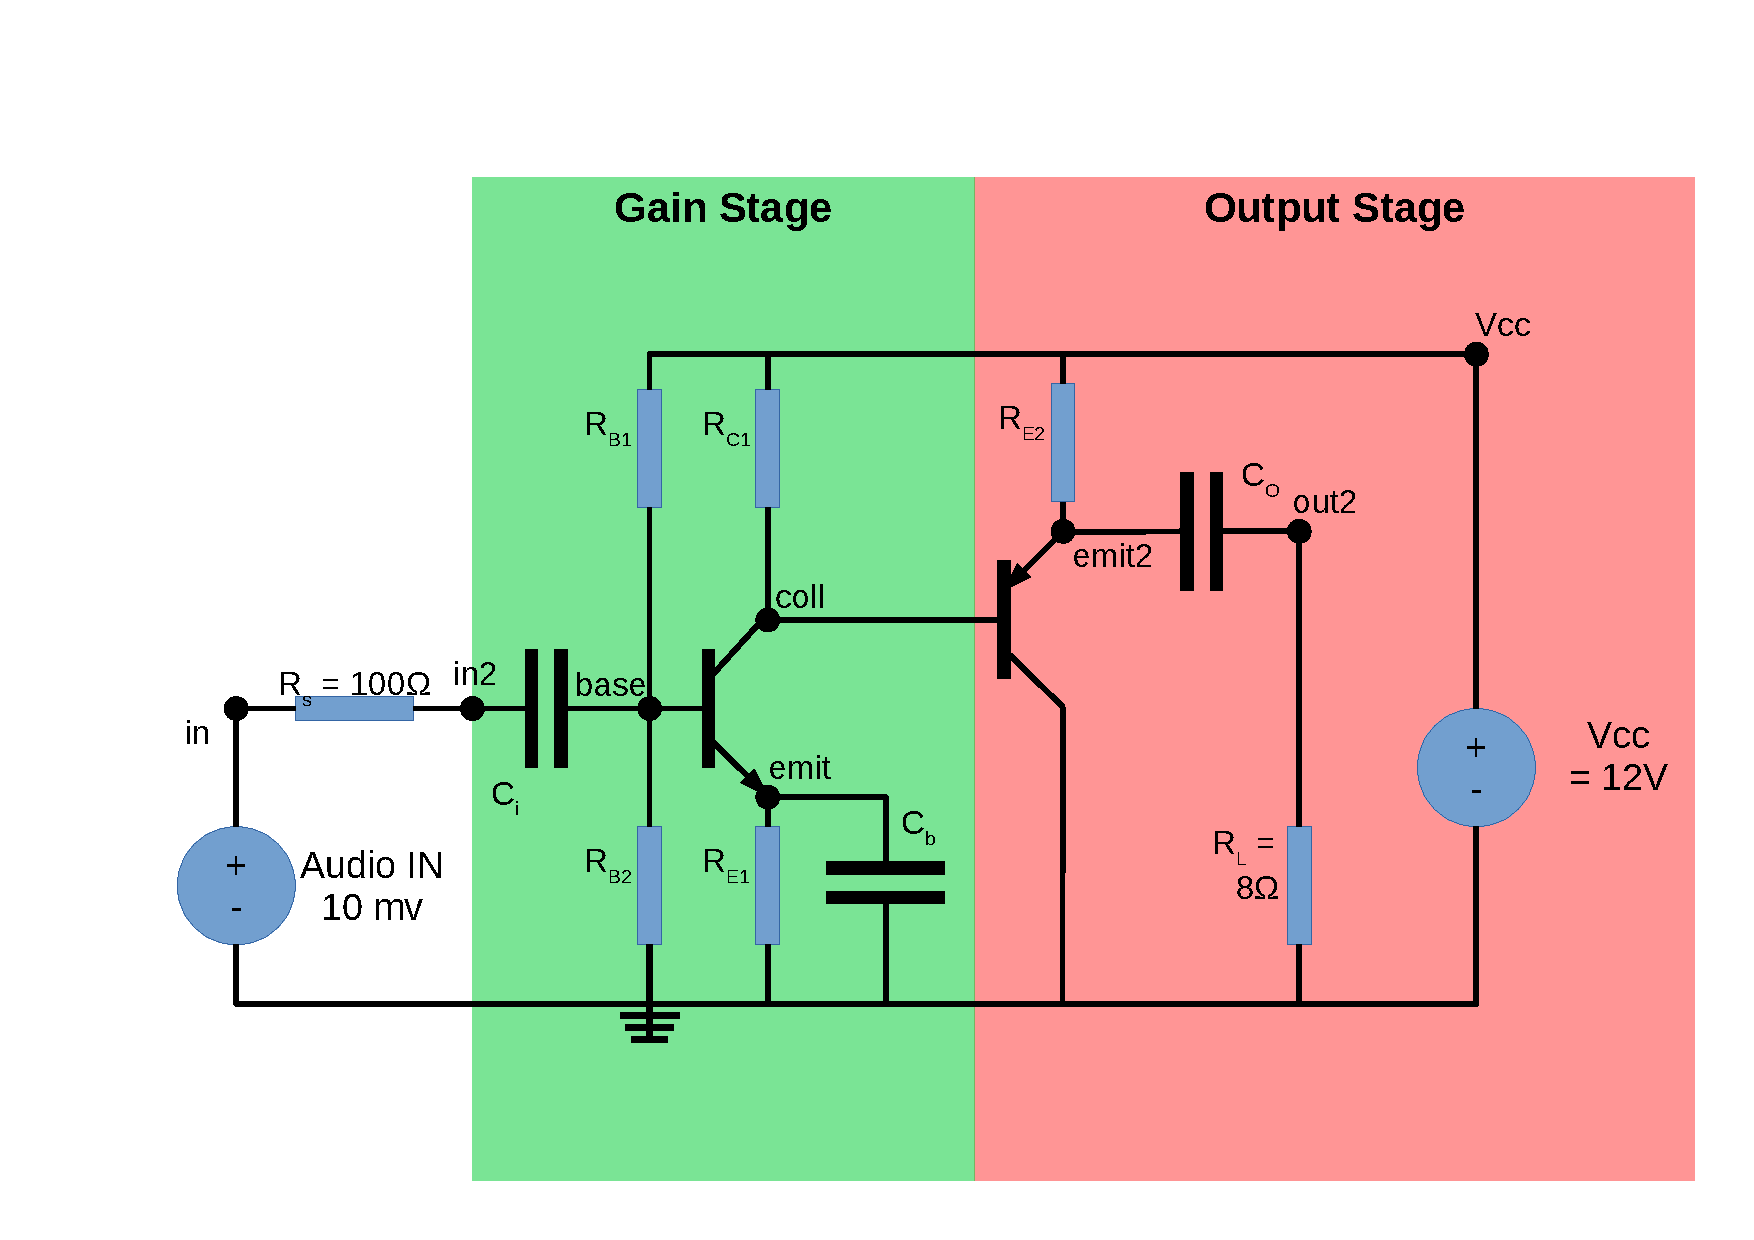
\includegraphics[width=0.9\linewidth]{./Circuit.pdf}
	\caption{T2 RC circuit.}
	\label{fig:rc}
\end{figure}

\paragraph{} It can be decomposed in wo main stages: the Gain Stage (in green)  and the Output Stage (in red).

\paragraph{} In the Gain Stage the original signal will be amplified. However, this amplified signal is not apropriate to be connected to our load (the speaker) due to it's high independance.

\paragraph{} Therefore, the signal goes through the Output Stage, that, due to it0s lowed independance, makes the signal suitable to be conected to the speake (which is connected in series).

\paragraph{} To perform the Theoretical Analysis we will look into the Gain and Output Stages separatelly.

\paragraph{} In Section 2 we will perform the Theortetical Analysis of the circuit, determining the operating point gain, inpendances and frequency response.

\paragraph{} In Section 3 we will obtain the simulation results to perform the Simulation Analysis.

\paragraph{} To conclude, we will draw our comparisons in Section 4 and lay our conclusions, looking into any possible differences and determining it's causes.

\paragraph{} In the table bellow we list the numerical values of the components used.

[LISTA DOS COMPONENTES]

\clearpage
